\let\negmedspace\undefined
\let\negthickspace\undefined
\documentclass[journal]{IEEEtran}
\usepackage[a5paper, margin=10mm, onecolumn]{geometry}
%\usepackage{lmodern} % Ensure lmodern is loaded for pdflatex
\usepackage{tfrupee} % Include tfrupee package

\setlength{\headheight}{1cm} % Set the height of the header box
\setlength{\headsep}{0mm}     % Set the distance between the header box and the top of the text

\usepackage{gvv-book}
\usepackage{gvv}
\usepackage{cite}
\usepackage{amsmath,amssymb,amsfonts,amsthm}
\usepackage{algorithmic}
\usepackage{graphicx}
\usepackage{textcomp}
\usepackage{xcolor}
\usepackage{txfonts}
\usepackage{listings}
\usepackage{enumitem}
\usepackage{mathtools}
\usepackage{gensymb}
\usepackage{comment}
\usepackage[breaklinks=true]{hyperref}
\usepackage{tkz-euclide} 
\usepackage{listings}
% \usepackage{gvv}                                        
\def\inputGnumericTable{}                                 
\usepackage[latin1]{inputenc}                                
\usepackage{color}                                            
\usepackage{array}                                            
\usepackage{longtable}                                       
\usepackage{calc}                                             
\usepackage{multirow}                                         
\usepackage{hhline}                                           
\usepackage{ifthen}                                           
\usepackage{lscape}
\begin{document}

\bibliographystyle{IEEEtran}
\vspace{3cm}

\title{9-9.3-15}
\author{AI24BTECH11003 - Badde Vijaya Sreyas}
% \maketitle
% \newpage
% \bigskip
{\let\newpage\relax\maketitle}

\renewcommand{\thefigure}{\theenumi}
\renewcommand{\thetable}{\theenumi}
\setlength{\intextsep}{10pt} % Space between text and floats


\numberwithin{equation}{enumi}
\numberwithin{figure}{enumi}
\renewcommand{\thetable}{\theenumi}


\textbf{Question}:\\
Find the equation of the tangent to the curve $y= \sqrt{3x-2}$ which is parallel to the line $4x-2y+5=0$. Also write the equation of the normal to the curve at the point of contact.


\solution
\begin{table}[h!]
	\centering
	\begin{tabular}[12pt]{|c|c|l|}
    \hline
	\textbf{Point} & \textbf{Position} & \textbf{Description}\\ 
    \hline
	\textbf{A} & $\myvec{x \\ y}$ & Unknown end of a diameter \\
    \hline 
	\textbf{B} & $\myvec{1 \\ 4}$ & Known end of diameter \\
    \hline
	\textbf{O} & $\myvec{2 \\ -3}$ & Center of the circle \\
    \hline   
    \end{tabular}

	\caption{Information}
	\label{tab:9-9.3-15}
\end{table}

From \eqref{eq:conic_quad_form} the curve can be rewritten as:
\begin{align}
    \vec{g}\brak{\vec{x}} = \vec{x}^\top \myvec{0&0\\0&1}\vec{x} + 2\myvec{\frac{-3}{2}\\0}\vec{x}+2
\end{align}
Now, since we know $\vec{m}$ already, we can use \eqref{eq:conic_tangent_mq} to find a point on the tangent, $\vec{q}=\myvec{x\\y}$.
\begin{align}
    \vec{m}^{\top}\brak{\vec{V}\vec{q}+\vec{u}}=0
\end{align}
\begin{align}
    \myvec{1\\2}^{\top}\brak{\myvec{0&0\\0&1}\vec{q}+\myvec{-\frac{3}{2}\\0}}=0\\
    y=\frac{3}{4}
\end{align}
Now with this value of $y$, and the equation of the curve,
\begin{align}
    \vec{q}=\myvec{\frac{41}{48}\\ \frac{3}{4}}
\end{align}
$\therefore$ From this point on the line, and the value of $\vec{m}$, the tangent can be written as:
\begin{align}
    \vec{X}=\myvec{\frac{41}{48}\\\frac{3}{4}} + \kappa \myvec{1\\2}
\end{align}
From \eqref{eq:line-school-normal}, the normal to the curve at the point of contact can be written as:
\begin{align}
	\vec{X_N}=\myvec{\frac{41}{48}\\\frac{3}{4}} + \gamma \myvec{-2\\1}
\end{align}
which can also be written as
\begin{align}
	\vec{X}=\frac{1}{48}\myvec{41\\36} + \kappa \myvec{1\\2} \\
	\vec{X_N}=\frac{1}{48}\myvec{41\\36} + \gamma \myvec{-2\\1}
\end{align}

\begin{figure}[h!]
\begin{center}
	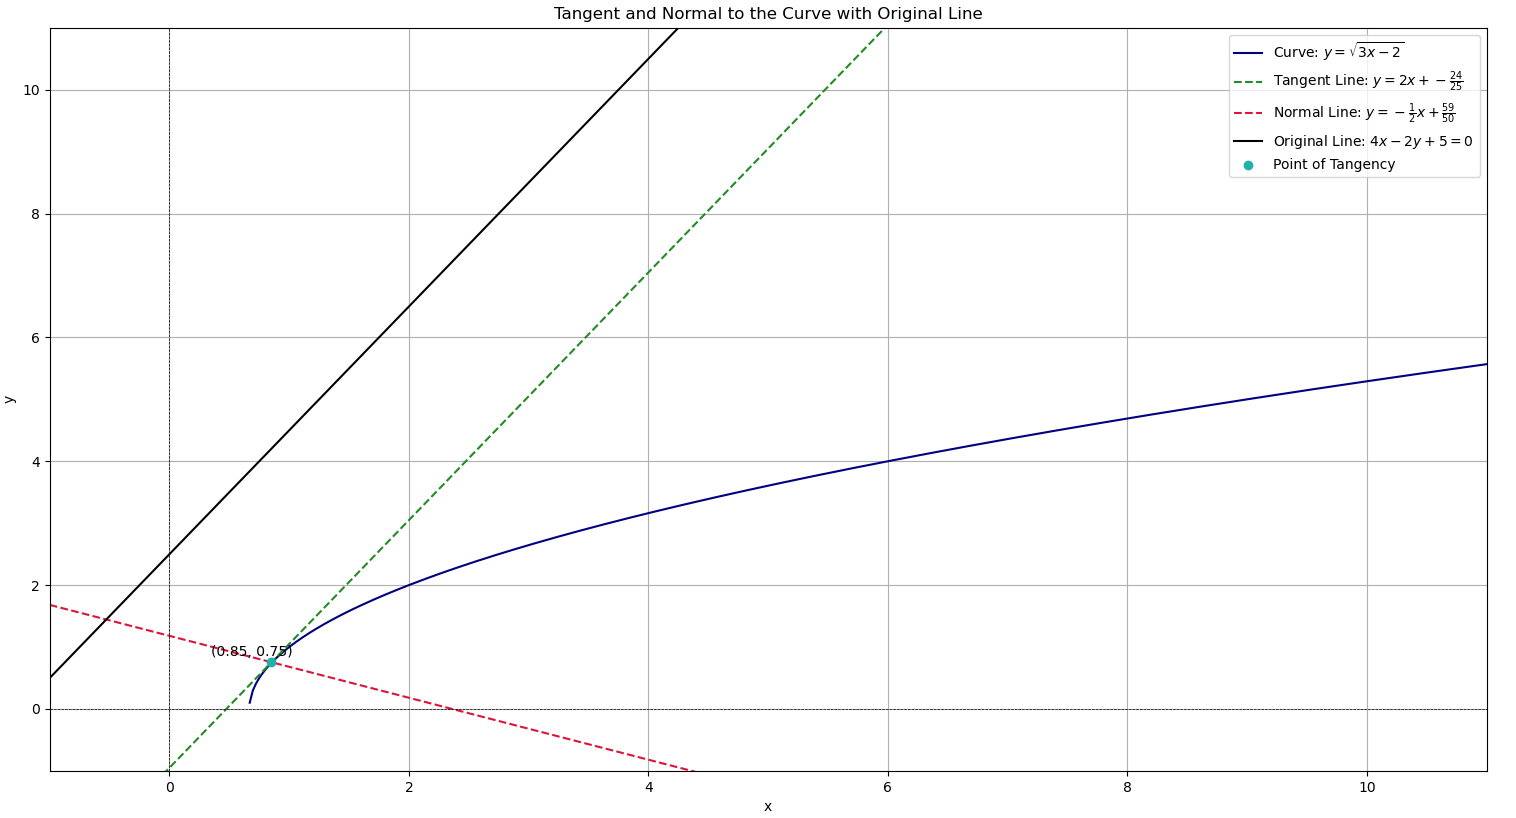
\includegraphics[width=0.9\textwidth]{figs/Figure_1.png}
	\caption{Lines and Curve}
	\label{fig:9-9.3-15 - Figure -1}
\end{center}
\end{figure}
\end{document}


